\chapter{New Material for Linear Algebra}
\chapterauthor{Jeff Yoshimi}

% TODO: Pictures for source-target representations

\subsection{The scalar and vector tracks}

% Compare https://youtu.be/Smav86u60FM?t=390 (from neurons to tokens, from weighted combinations of scalars to weighted combinations of vectors)

%To get to the next belt level, you have to deal with this kind of thing, and so train your brain to deal with it.

The book  can be thought of as involving two tracks: a `scalar' and a `vectorized' track. In the scalar track, we think of all operations from the standpoint of individual neurons and their values. We index weights using a source-target structure. In Simbrain, the focus is mostly on separately presented nodes. We use vectors and matrices to understand many ideas conceptually, but we do not make heavy use of matrix products or matrix algebra. This is much more accessible to beginning students, and is sufficient to teach an entire class. Indeed, this has been the way the book was structured and is the main way Simbrain 3.0 works. This supports the main thrust of the book and Simbrain, making neural networks easy enough to use without any math background at all (there is math to learn, but it is self contained). 
% Source target entails a different representation of matrices

However, this is not how things are done by most professionals working on neural networks in industry, and most academics as well (ch 1 taxonomy). For any serious work, we must move to the vectorized approach. Everything becomes more concise, and runs more efficiently on high performance performance computers. This requires a change in thinking, a way of seeing and thinking about these problems in terms of matrices, vectors, and tensors, often seeing datasets and batches in new ways, almost as tubes of information that get transformed. The focus here is on vectors, matrices, and higher rank tensors, and on applying linear algebra methods directly to these structures. The weights are now indexed using a target-source scheme. The basic objects are mostly matrices, and matrix products--especially multiplications of matrices by column vectors--are the basic operations. In Simbrain 4.0 we have been and are making efforts to make this mode of thinking more intuitive. As of now, there is very little in this format in the book, but we are in the process of adding chapters and sections that present that point of view. Ultimately the hope is to have enough material that a more advanced course could be done entirely from that point of view.

One downside of this is that the indexing changes depending on what you read, but we hope this downside can be an upside. The main book allows a non-math approach, but those going to the target-source point of view must also develop an ability to switch between representations, to see it both ways, which is more complex cognitively but in a way that suits the more advanced mind sets. Many problems are like that, allowing for multiple representations.

% Define shape of matrix
% Transposes.  Also address in line vectors and whether they need the transpose. There's this weird situation. In simbrain and in general, the default is columns.   But in a book, the default is row.  So to show column we do transose operator. But if bold face alone, it is colulmn

\subsection{Graphical conventions}

To think in terms of vectors, we need to bridge between conventional linear algebra notation, and conventional neural network representations, as in Simbrain.  We need a template for mentally moving back and forth between these ways of thinking.  

The first thing to do is get clear on the shape of the matrix. Remember, we are using an ``output-input'' representation.  It feels backwards but it's how it's done.  So, in figure \ref{linalgToSimbrain}, start on the right with Simbrain.  Count the number of outputs, then the number of inputs. Then we have an output-input matrix.  So $3$, $2$, and a $3 \times 2$ matrix.

\begin{figure}[h]
\centering
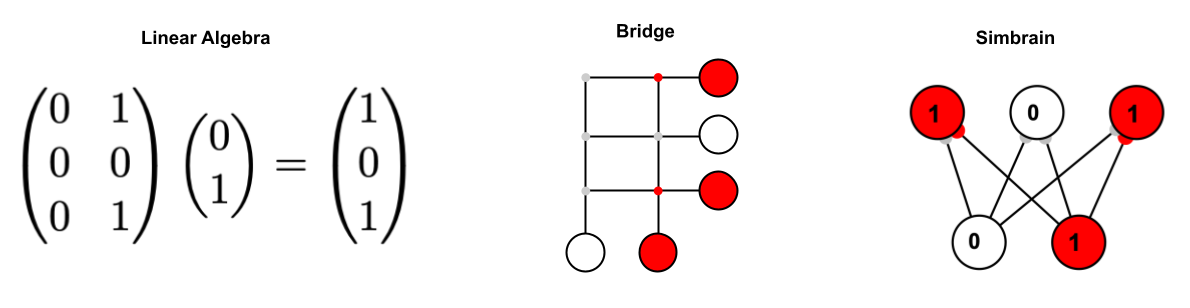
\includegraphics[width=0.75\textwidth]{images/LinalgToSimbrainReps.png}
\caption[Jeff Yoshimi.]{A set of images to help link standard visual representations in linear algebra (left) with standard visual representations of neural networks (right), via the intermediate representation in the middle. }
\label{linalgToSimbrain}
\end{figure}

Figure \ref{linalgToSimbrain} is an effort to bridge this gap. On the left is a standard matrix product, $\mathbf{W} \mathbf{x} = \mathbf{y}$.  This is how forward propagation of an input vector through a weight matrix is usually understood. The weight matrix is $\mathbf{W}$, the input is $\mathbf{x}$, and the output is $\mathbf{y}$. We think of the matrix as operating on the column vector to produce a new column vector.   

% need a transpose section
Here is how I suggest you think about this to connect it up to intuitions about neural networks.  Think of the column vector $\mathbf{x}$ as being rotated 90 degrees or transposed to become a row vector (imagine grabbing the vector by the $1$ and pulling it up and to the right). Now mentally take this row and move it to the bottom of the weight matrix, as in the middle panel of  \ref{linalgToSimbrain}. The weight matrix and the output vector stay in the same orientation.  The fan-out weight vectors from the input are shown as vertical lines, and the fan-in weight vectors to the output are shown as horizontal lines. Now we can easily ``follow'' the activations upwards as activity is propagated. 
% The bridge is pretty close to the new simbrain rep. Show that?
% Note there are other reps too, like the points in a space rep.

I like to think of the input vector as being dotted with each fan-in weight vector on the outputs to produce the entries of the output vector.

To go from the bridge to the standard Simbrain representation in the right panel we now leave the inputs in place, and imagine the outputs being rotated 90 degrees and moved to the top, and imagine the weights kind of following along. Hopefully you can just see it. 

In Simbrain 4.0, we have designed the representation of activation vectors and weight matrices to follow the ``bridge'' concept above as closely as possible.  See figure \ref{simbrain4_ff23}.

\begin{figure}[h]
\centering
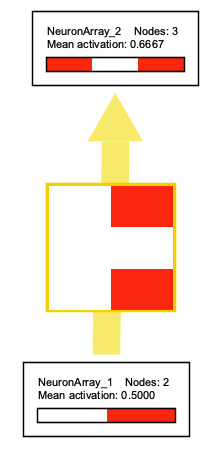
\includegraphics[width=0.15\textwidth]{images/simbrain4_ff_2_3.png}
\caption[Jeff Yoshimi.]{Graphical conventions for activation vectors and weight matrices in Simbrain 4. }
\label{simbrain4_ff23}
\end{figure}
%
%Also just a thought on how to think about the weight matrices. Their shape is target-source, or output-input. So if we have a 3-5-2-1 network in terms of node layers, we have three weight matrices. Their shapes are:
%
%5x3
%2x5
%1x2
%
%So you would pass a list of the form [5x3, 2x5, 1x2] to your function. Remember, weight matrices on the left are multiplied by input and activations vectors on the right.I find this pretty counter-intuitive and takes me a lot of practice to think in this “output-input” way.  I want to read left-to-right input-to-output but the standard conventions with matrix product reverse this...

